\subsection{YOLOv8}
\begin{frame}{}
    \LARGE Object Detection: \textbf{YOLOv8}
\end{frame}

\begin{frame}[allowframebreaks]{YOLOv8}
    \begin{figure}
        \centering
        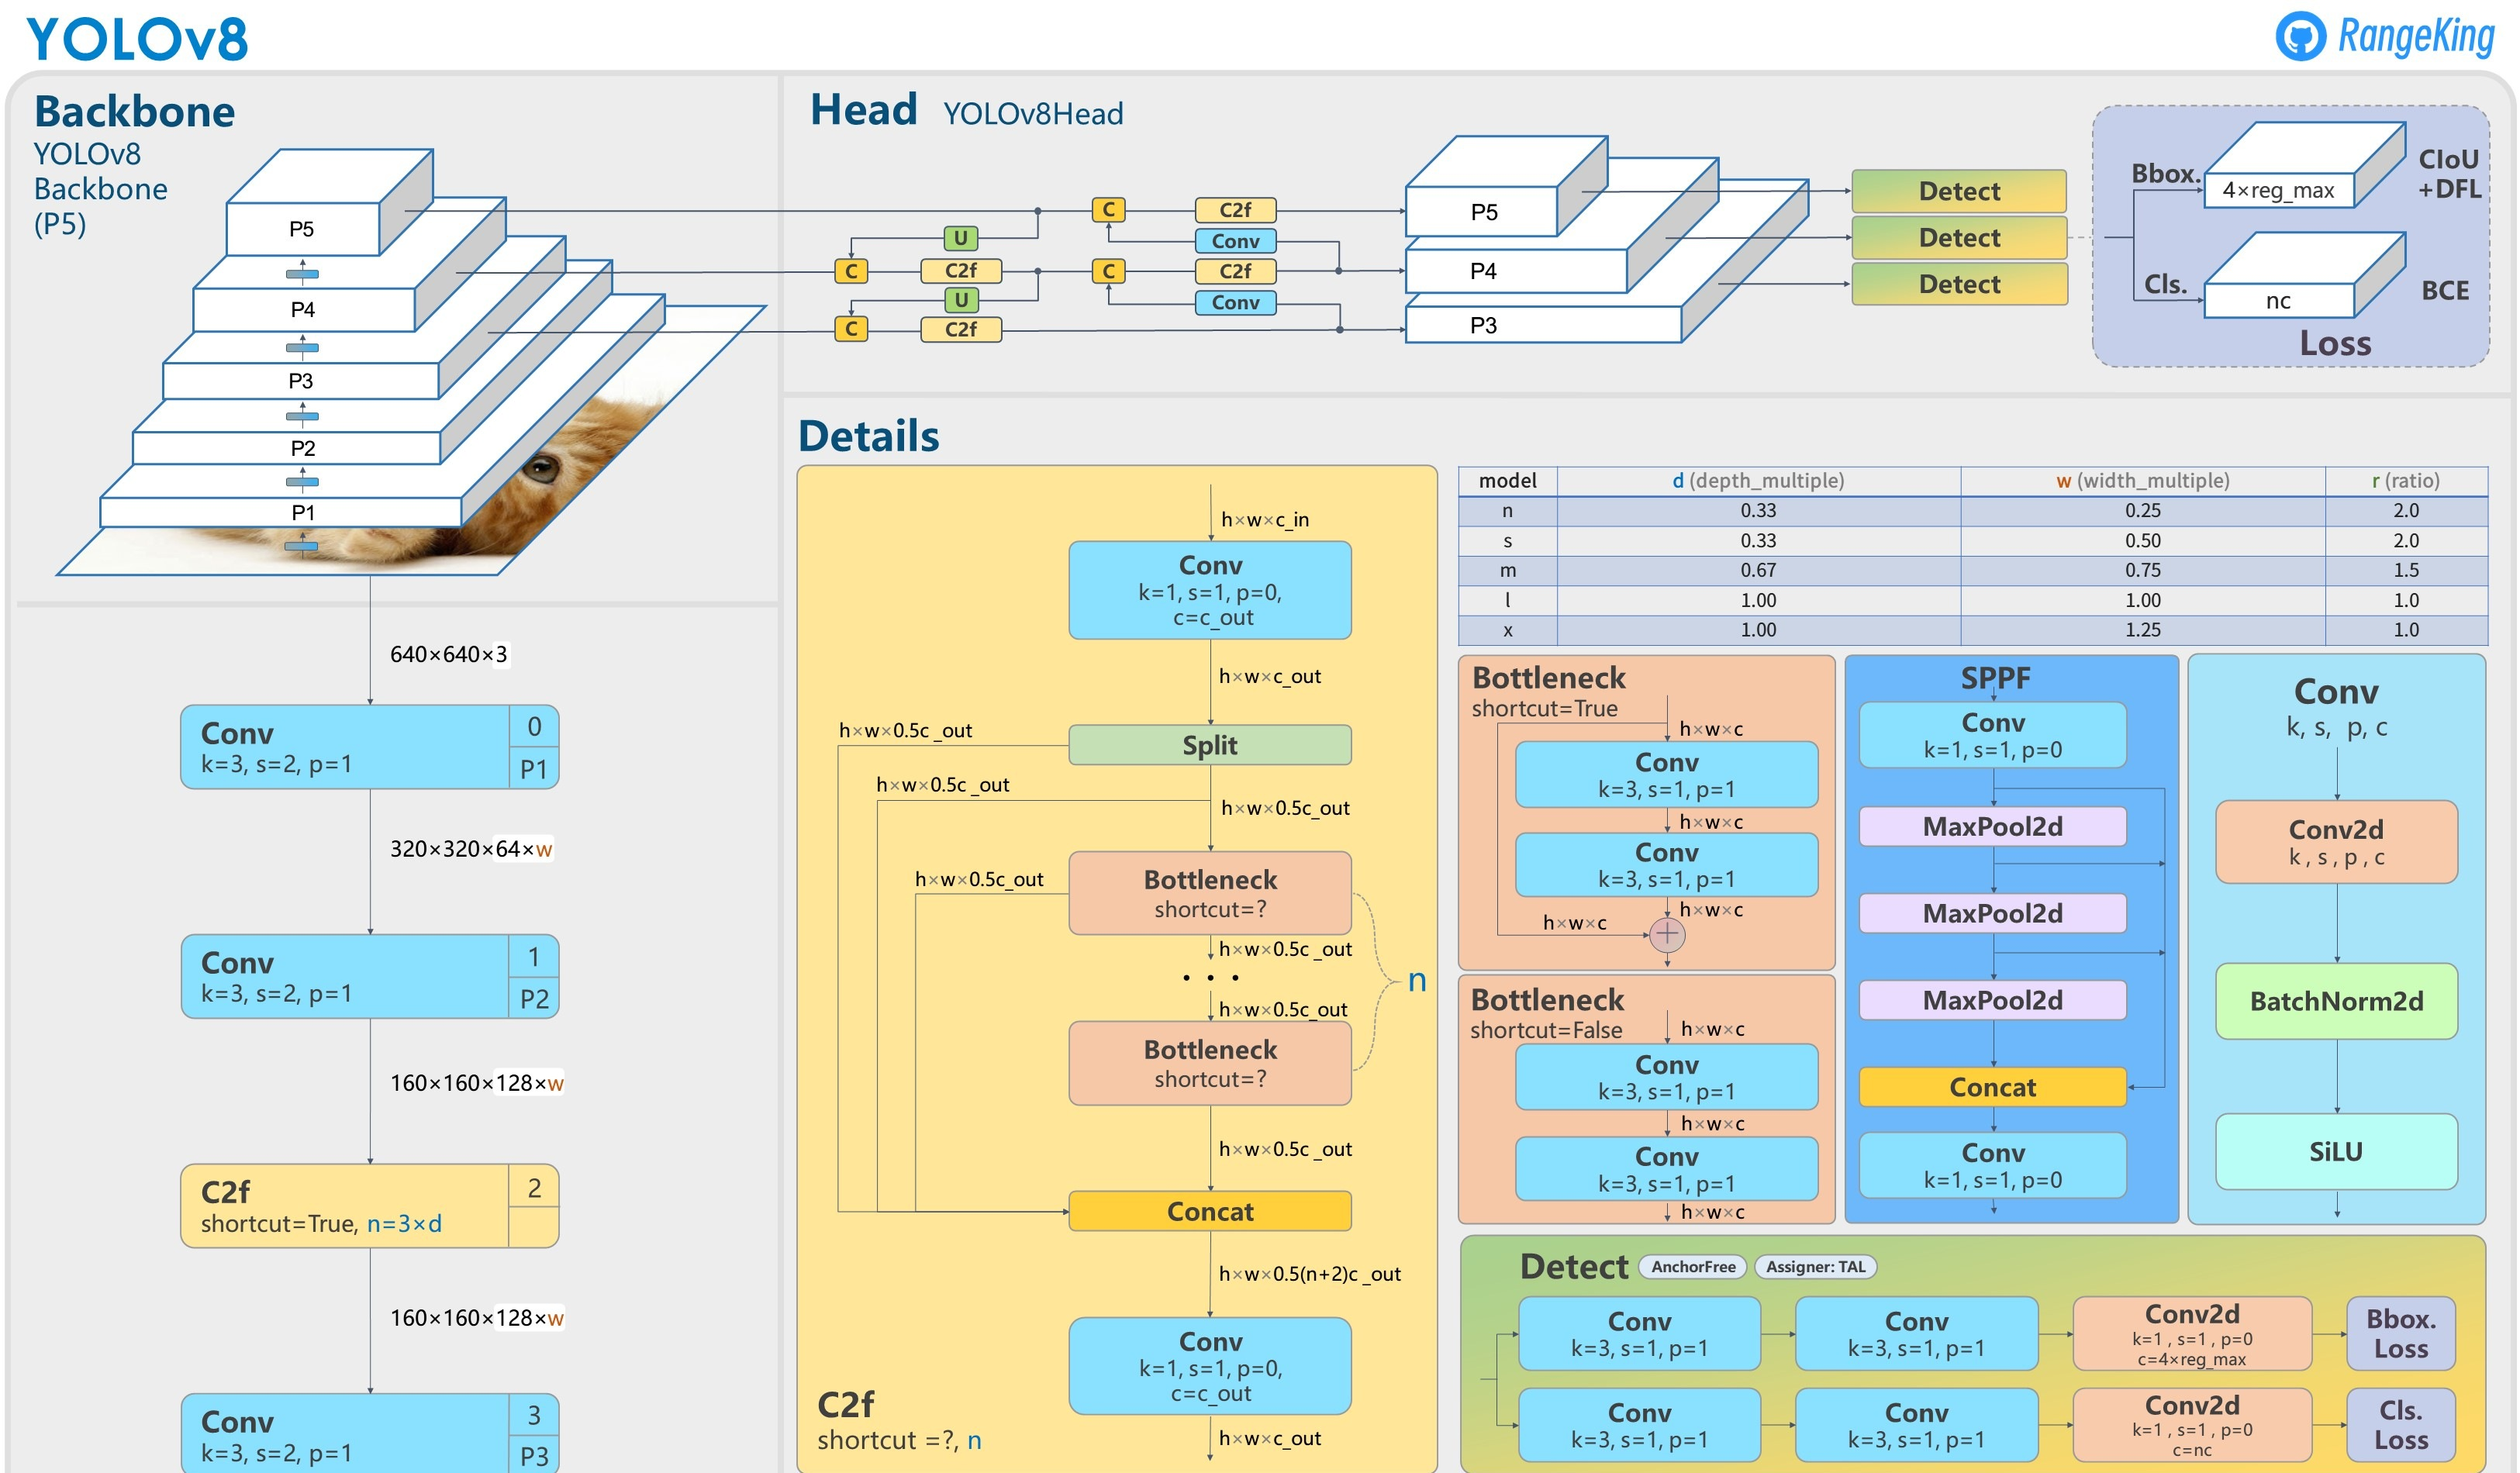
\includegraphics[width=1.0\textwidth,height=0.80\textheight,keepaspectratio]{images/object-detect/yolov8_architecture_rangeking_overview.jpg}
        \caption*{\scriptsize C2f replaces YOLOv5's C3; the anchor-free \texttt{Detect} head is decoupled, with no objectness branch. Source: YOLOv8 structure diagram by GitHub user RangeKing, ultralytics/ultralytics issue \#189, 2023 (free reuse).}
    \end{figure}
\framebreak
    \begin{figure}
        \centering
        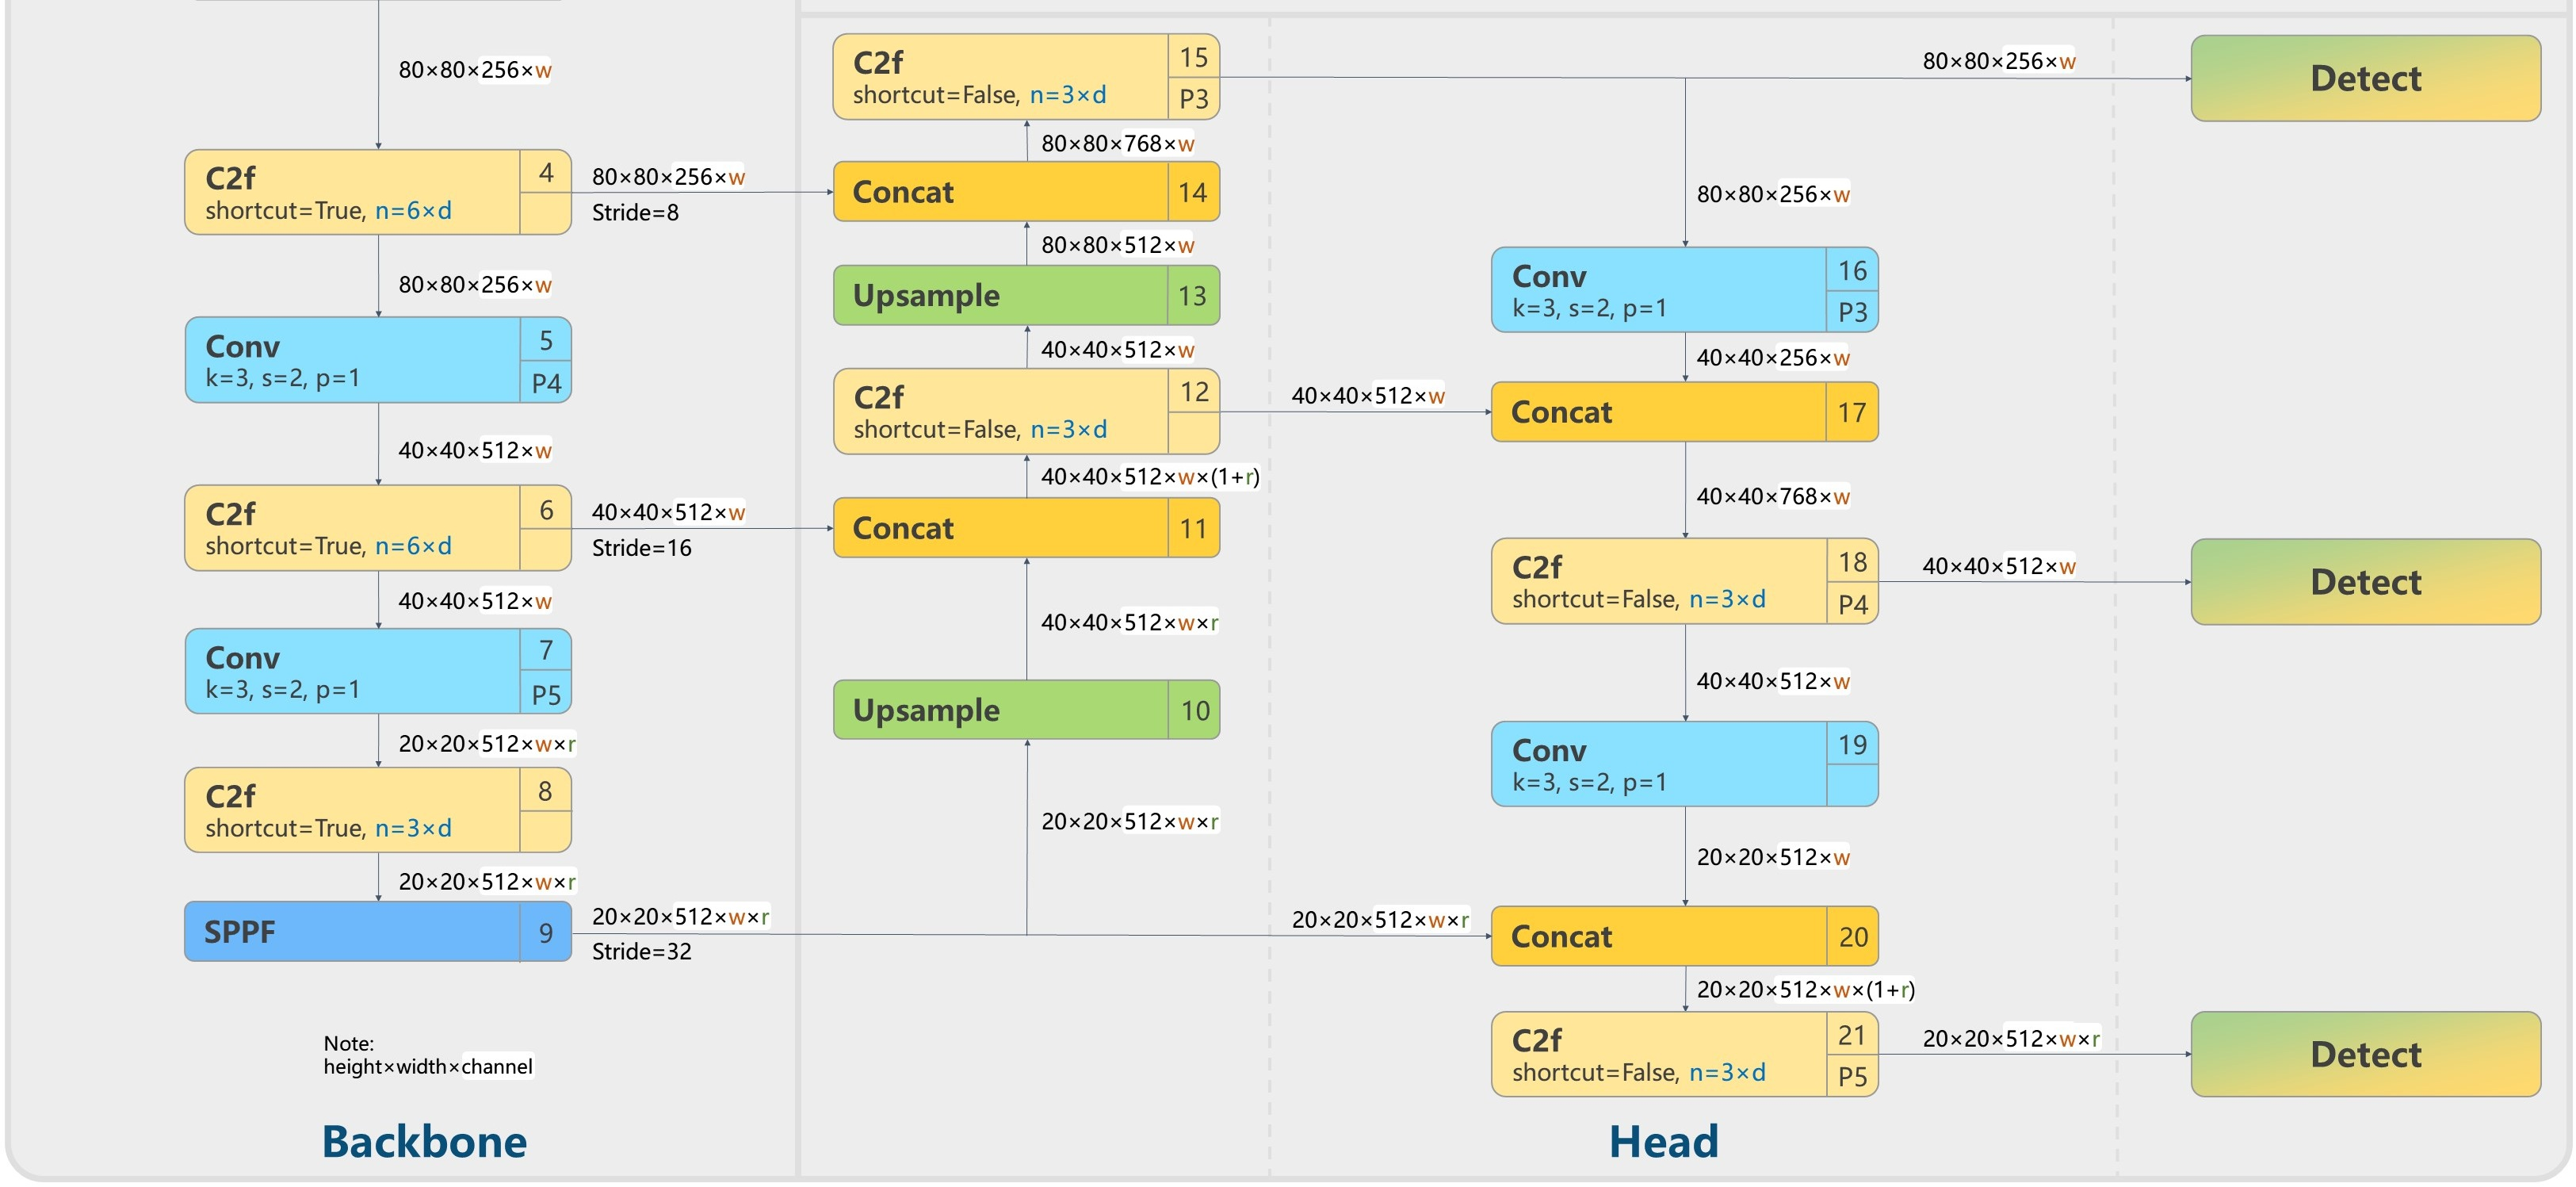
\includegraphics[width=0.95\textwidth,height=0.74\textheight,keepaspectratio]{images/object-detect/yolov8_architecture_rangeking_layers.jpg}
        \caption*{\scriptsize The 22 layers in full: backbone (0--9) into the PAN-style head (10--21), feeding three \texttt{Detect} heads at strides 8, 16 and 32. Same source as the previous slide.}
    \end{figure}
\framebreak
    \textbf{YOLOv8 (2023) Highlights:}
    \begin{itemize}
        \item \textbf{Anchor-free} detection architecture
        \item CSP backbone, FPN+PAN neck
        \item One codebase for detection, instance segmentation, pose estimation and classification
        \item COCO mAP from 37.3 (YOLOv8n) to 53.9 (YOLOv8x); YOLOv8l gives 52.9 mAP at 2.39\,ms per image on an A100 with TensorRT
        \item Strengths: multi-task capabilities, ease of use, segmentation support
        \item Challenges: small/clustered object detection remains difficult
    \end{itemize}
\end{frame}